\section{Arquitectura VO}

\subsection{Arquitectura VO según IOA}

\begin{frame}
\frametitle{Arquitectura VO según VOA}
El VO's es un framework que ayuda a resolver distintos
problemas que enfrenta la comunidad astronómica a lo largo del mundo.  Uno de
los problemas está relacionado al acceso a los datos, por lo que en IVOA
diseñaron tecnologías y estándares formalmente definidos, que permitan el de
acceso unificado y transparente a distintos servidores con datos astronómicos.

El beneficio que conlleva es considerable, ya que estos
estándares, protocolos, tecnologías y arquitectura, ayudan a la comunidad al
proceso de creación de servicios, portales web, aplicaciones de escritorio,
etc. Todo visto del punto de vista de ingeniería de software.
\end{frame}

\begin{frame}
\frametitle{Arquitectura Nivel 2}
\begin{multicols}{2}
\begin{itemize}
    \item \textbf{Capa de recursos}:
          compilado de datos astronómicos provenientes de distintos instrumentos.
    \item \textbf{Capa de usuarios}:
          investigadores que buscan consumir datos.
    \item \textbf{Capa intermedia}:
          es la capa que permite conectar las dos
          capas anteriores de manera transparente para los investigadores.
          Esta interacción se puede llevar a cabo buscando u obteniendo datos.
\end{itemize}

\begin{figure}[h!t]
    \centering
    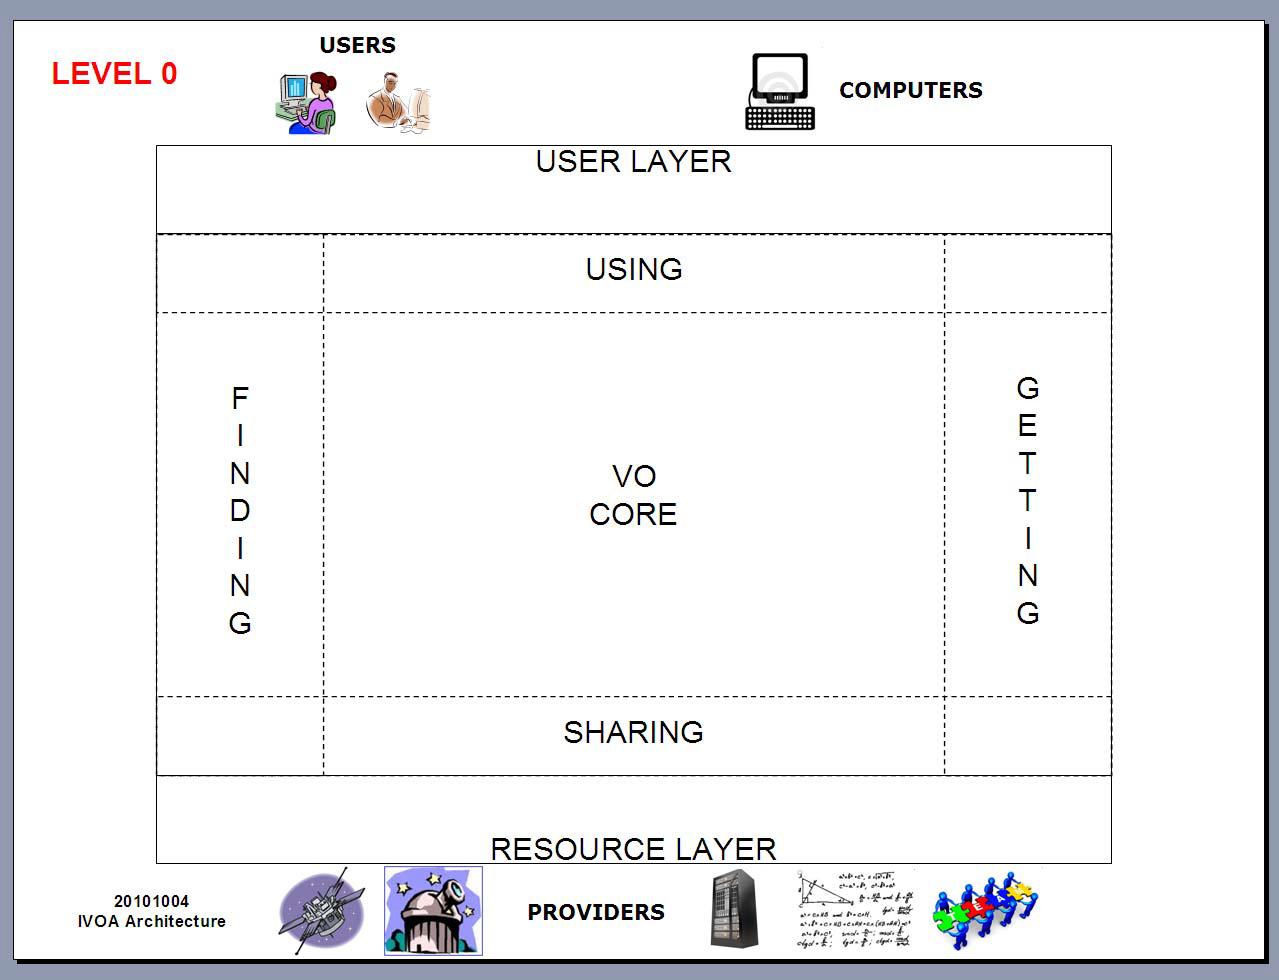
\includegraphics[width=0.5\textwidth]{img/arquitectura_0.png}
    \caption{Arquitectura Nivel 0}
    \label{fig:nivel0}
\end{figure}

\end{multicols}
\end{frame}


\begin{frame}
\frametitle{Arquitectura Nivel 1}
\begin{multicols}{2}

\begin{itemize}
    \item \textbf{Capa de recursos}:
          está compuesto de colección de datos y provenientes de distintos
          servidores.
    \item \textbf{Capa de usuarios}:
          un consumidor puede querer acceder a los datos desde un navegador,
          escritorio, o mediante un script.
    \item \textbf{Capa intermedia}:
          crea un framework para compartir los datos, compuesto por VOQL,
          Data Models, Semantics, Formats.
\end{itemize}

\begin{figure}[h!t]
    \centering
    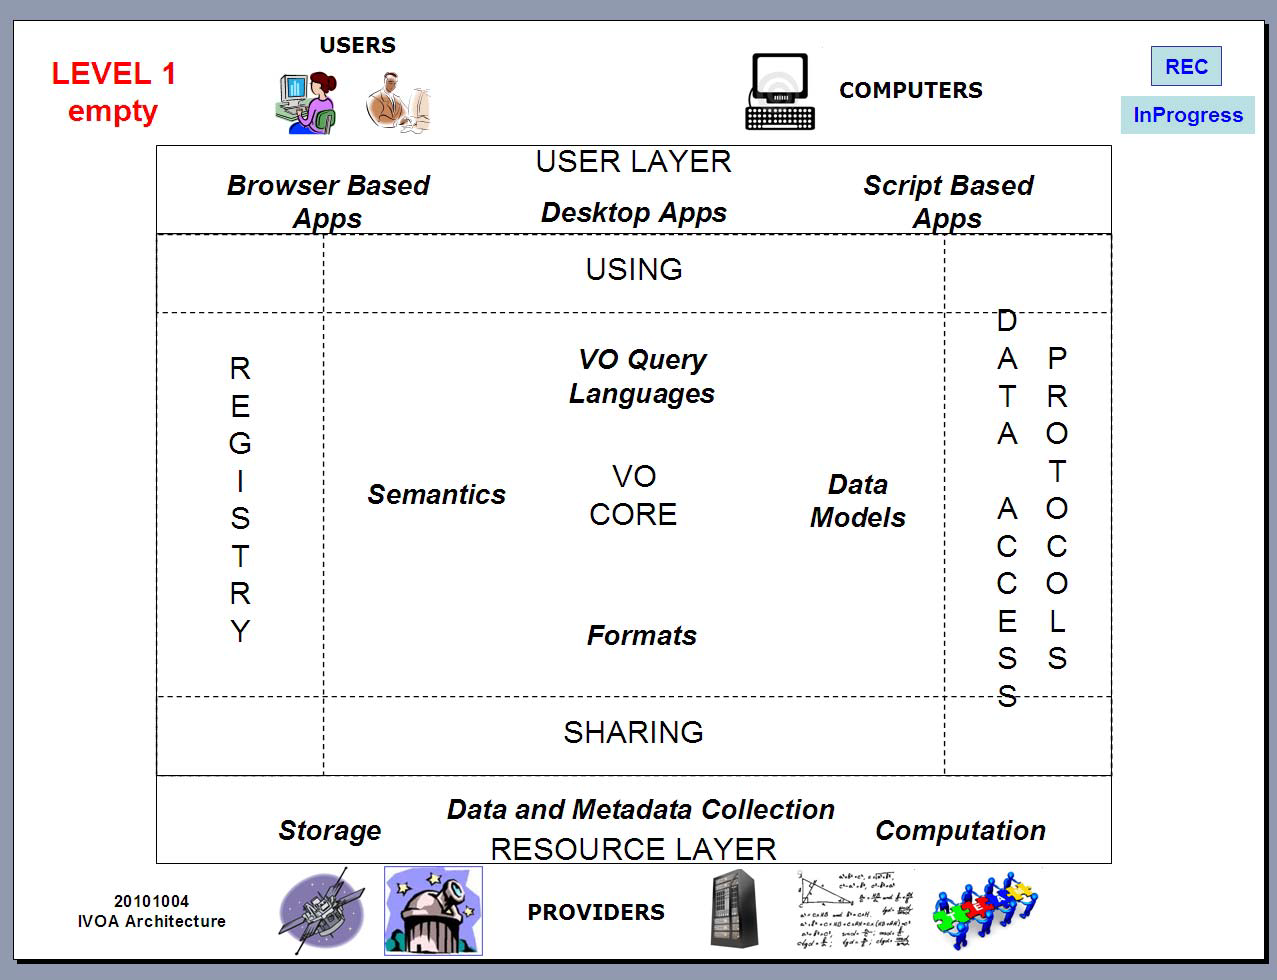
\includegraphics[width=0.5\textwidth]{img/arquitectura_1.png}
    \caption{Arquitectura Nivel 1}
    \label{fig:nivel1}
\end{figure}
\end{multicols}
\end{frame}

\begin{frame}
\frametitle{Arquitectura Nivel 2}
\begin{multicols}{2}

La arquitectura nivel 2 es lo que se entiende por un VO regido por estándares
y protocoloes de IVOA.
La idea de esta figura es seccionar cada estándar relacionándolo específicamente
a la capa a la cual pertenece.


\begin{figure}[h!t]
    \centering
    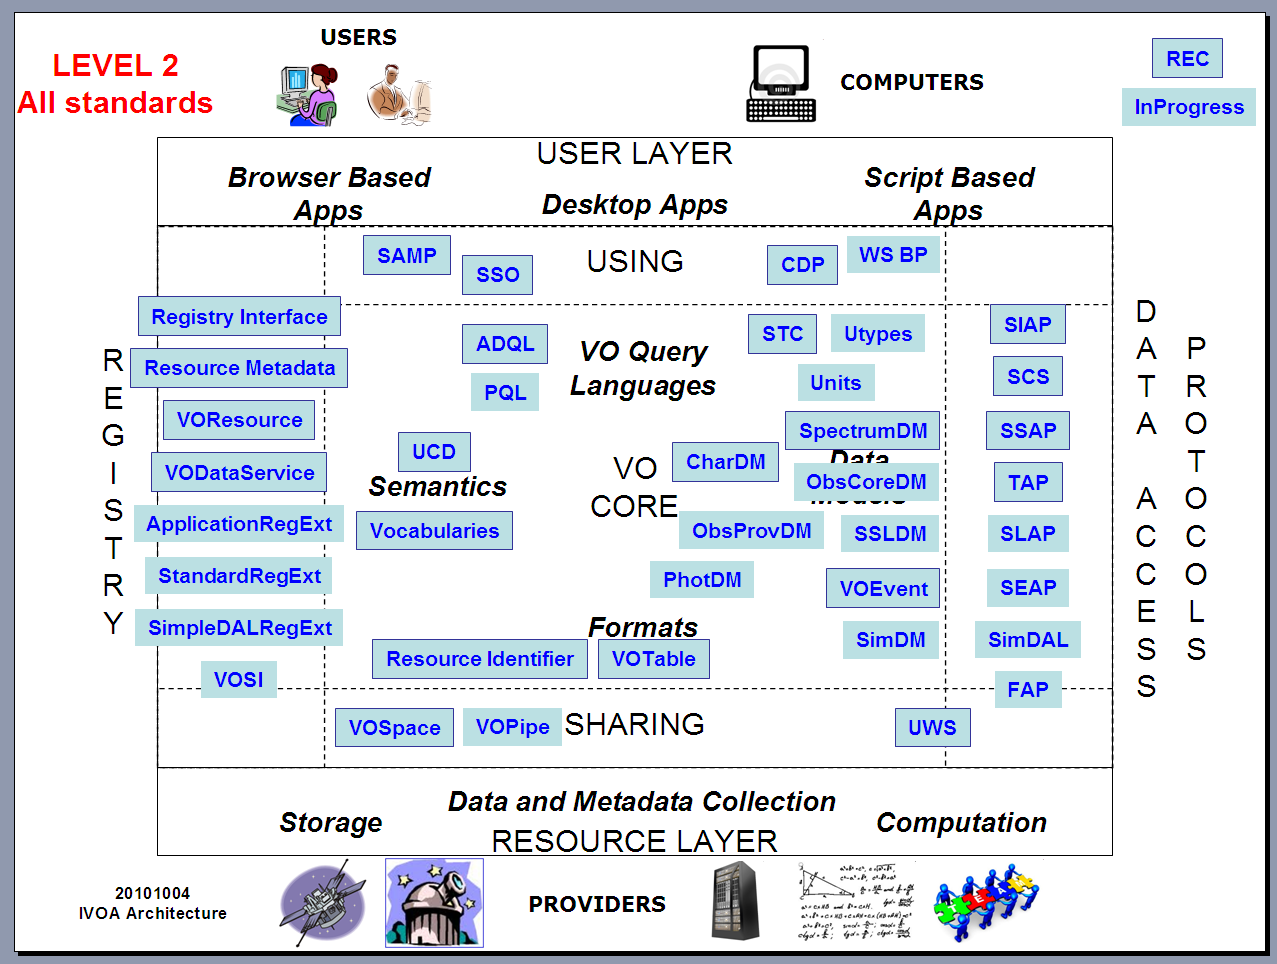
\includegraphics[width=0.5\textwidth]{img/arquitectura_2.png}
    \caption{Arquitectura Nivel 2}
    \label{fig:nivel2}
\end{figure}

\end{multicols}
\end{frame}
